

	\documentclass[15pt]{article}
  \usepackage[T1]{fontenc}
  \usepackage[utf8]{inputenc}
  \usepackage[polish]{babel}
  \usepackage{indentfirst}
  \usepackage{xcolor}
  \usepackage{graphicx} 
  \usepackage{subcaption}
  
  \usepackage{fancyhdr}
  \usepackage{lastpage}
  \usepackage[margin=1.45in]{geometry}

  \pagestyle{fancy}
  \fancyhf[HR]{}
  
  \AtBeginDocument{%
    \addtocontents{toc}{\protect\thispagestyle{empty}}%
    \addtocontents{lof}{\protect\thispagestyle{empty}}%
  }
  
  \cfoot{Strona \thepage \hspace{1pt} z \pageref{LastPage}}
  
  \author{Mateusz Milewski}
  \title{\textbf{Specyfikacja Implementacyjna projektu indywidualnego ,,JapanApp''}}
  \frenchspacing
  \begin{document}
  \maketitle
  \tableofcontents
  \clearpage
  \section{Informacje ogólne}
  \subsection{Opis przekrojowy}
  Dokument ten jest specyfikacją implementacyjną aplikacji ,,JapanApp''. Zostały tutaj zawarte najistotniejsze informacje dotyczące sposobu implementacji tej aplikacji. W celu dobrego zrozumienia całego dokumentu, poniżej został zamieszczony krótki opis działania całej aplikacji.
  \newline
  \newline
  Aplikacja będzie aplikacją edukacyjną, której celem jest nauka alfabetu japońskiego. Aplikacja docelowo ma znajdować się w ,,Google Play'', gdzie użytkownik powinien mieć dostęp do jej pobrania. Po uruchomieniu aplikacji, wypełniając cały ekran telefonu, pojawi się okno z menu głównym. Użytkownik następnie wybierze tryb gry ,,GuessIt'' lub ,,DrawIt''. Po zatwierdzeniu przełączona zostaje scena menu na scenę z wyborem systemu znakowego. Użytkownik dokonuje kolejnego wyboru i następnie wyświetla się scena z rozgrywką odpowiednią do poprzednich decyzji. Tryb ,,GuessIt'' polega na odgadnięciu jaki znak jest wyświetlony, natomiast ,,DrawIt'' polega na narysowaniu odpowiedniego znaku. Oba tryby kończą się wyświetleniem sceny z podsumowaniem. Po podsumowaniu aplikacja wraca do sceny z menu głównym, gdzie użytkownik może ponownie wybrać rozgrywkę albo sprawdzić informacje od twórców.
  
  \subsection{System docelowy}
  Docelowy system, na którym aplikacja będzie funkcjonowała, jest Android. Aplikacja będzie wspierana na każdym urządzeniu, które posiada wersję Androida od 4.1 wzwyż. 
  \subsection{Język}
  Aplikacja pisana będzie w Javie, w wersji 8.
  \subsection{Konwencja nazewnictwa} 
  Nazewnictwo klas, metod i pól zostaje utrzymane w konwencji:
  \begin{itemize}
    \item Nazwy klas rozpoczynać się będą wielką literą.
    \item Nazwy metod i atrybutów klas rozpoczynać się będą od małej litery. W przypadku gdy nazwa będzie miała składać się z więcej niż jednego słowa to utrzymana zostaje konwencja ,,camelCase'', czyli każde kolejne słowo będzie rozpoczynało się od wielkiej litery.
  \end{itemize}
  
  \subsection{Wykorzystywane narzędzia}
  Cały program pisany będzie w środowisku ,,Android Studio''. Oferuje ono wiele przydatnych narzędzi do stworzenia tej aplikacji. Główną funkcjonalnością, która zostanie wykorzystana tym projekcie jest edytor graficzny, który automatycznie generuje kod z rozszerzeniem xml. Oprócz samego edytora graficznego w programie zostanie użyta biblioteka ,,Canvas'', również pozwalająca rysować elementy graficzne. W celu tworzenia testów jednostkowych zostanie użyta biblioteka Junit w wersji 4. 
  
  \subsection{System kontroli wersji}
  Cały projekt będzie korzystał z systemu kontroli wersji GitHub.
  Commity oznaczające kamienie milowe będą oznaczane tagami,
  których nazwa będzie nawiązywać do funkcjonalności, którą udało się uzyskać. 
  \newline 
  \newline
  np. udało się stworzyć ekran do rysowania palcem, odpowiadający mu tag będzie mieć postać $FingerPathing\_1.$
  \section{Opis pakietów}
  Aplikacja ta to nie będzie bardzo rozbudowany projekt. Nie wliczając pakietów tworzonych automatycznie poprzez Gradle'a, to cała zawartość programu zamknie się w trzech pakietach - main, images oraz test. 
  
  
  \subsection{Main}
  Będzie to pakiet zawierający zarówno wszystkie pliki źródłowe klas, jak i wszystkie pliki z rozszerzeniem xml reprezentujące odpowiednie sceny w aplikacji.
  
  \subsection{Images}
  Pakiet ten zawierać będzie wszystkie pliki reprezentujące wygląd znaków z języka japońskiego. Pliki te będą zawierały rozszerzenie .png lub .jpg.
  \subsection{Test}
  W tym pakiecie znajdować sie będą wszystkie pliki związane z testowaniem aplikacji. 
  \newpage
  \section{GUI}
  Aplikcja oferować będzie możliwość płynnego poruszania się po kolejnych scenach. Efekt ten uzyskany zostanie poprzez stworzenie kilku (wypisane poniżej) scen reprezentowanych w programie, poprzez ,,Activity'', które następnie będą przełączały się między sobą po wciśnięciu odpowiednich przycisków. 
  
  \subsection{Scena menu głównego}
  Pierwsza scena (rysunek 1a), którą ujrzymy po uruchomieniu aplikacji. Scena ta składać się będzie z 3 przycisków, ustawionych jeden pod drugim w odpowiedniej kolejności:
  \begin{itemize}
    \item ,,DrawIt'' -- przycisk po kliknięciu uruchamiał będzie funkcję przenoszącą do sceny z wyborem systemu znakowego. Dodatkowo, po jego kliknięciu zostanie zapisana informacja o tym, że użytkownik chce grać w trybie ,,DrawIt''.
    \item ,,GuessIt'' -- przycisk analogiczny w działaniu z tym wyjątkiem, że zapisywać będzie wybór trybu jako ,,GuessIt''.
    \item ,,Credits'' -- po jego wciśnięciu zostanie uruchomiona funkcja zmieniająca na scenę z informacjami od twórców.
  \end{itemize}
  
  \begin{figure}[h!]
    \centering
    \begin{subfigure}[b]{0.35\linewidth}
      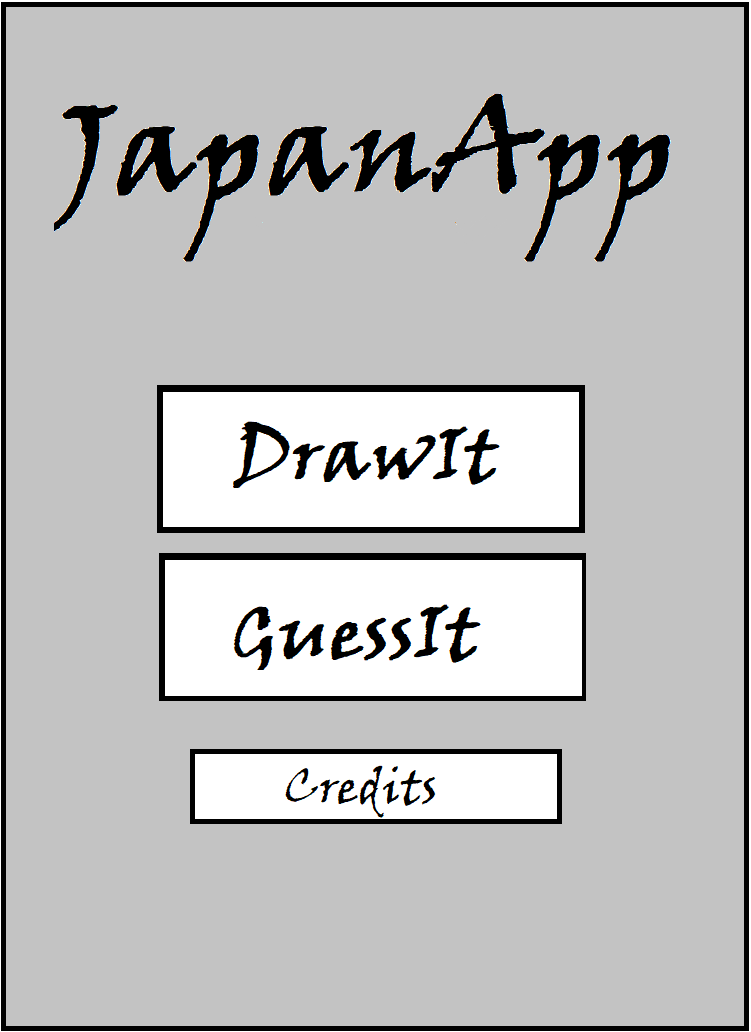
\includegraphics[width=\linewidth]{menu.png}
      \caption{Wizualizacja okna z menu głównym.}
      \label{rysunek1}
    \end{subfigure}
    \begin{subfigure}[b]{0.35\linewidth}
      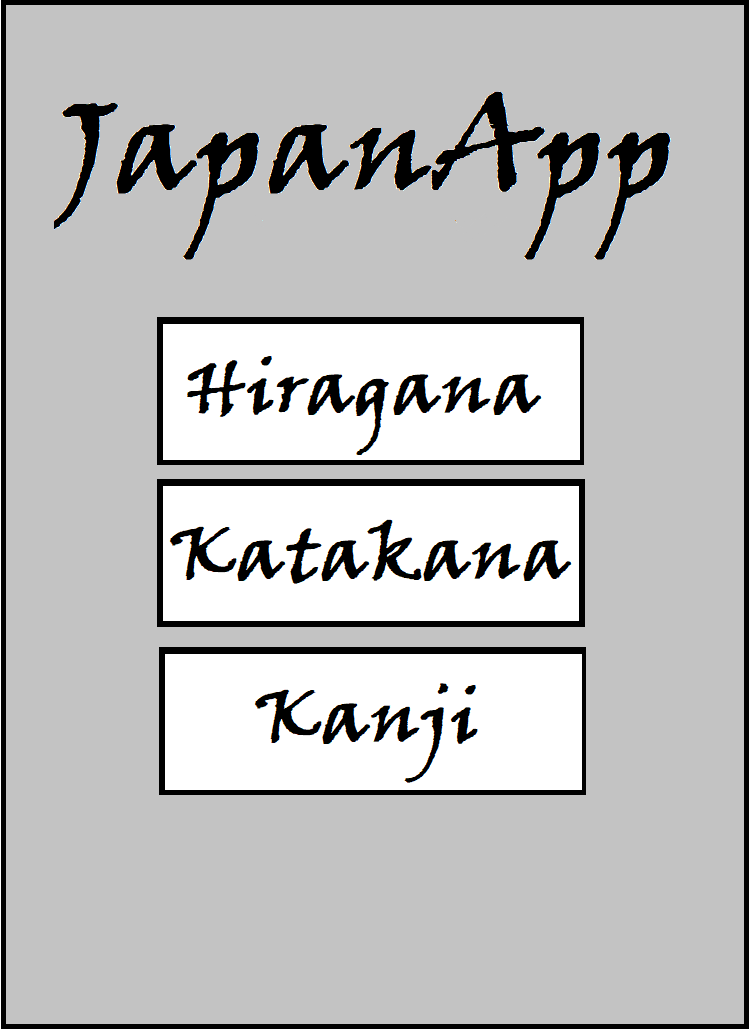
\includegraphics[width=\linewidth]{chose.png}
      \caption{Wizualizacja okna z wyborem systemu znakowego.}
      \label{fig:rysunek2}
    \end{subfigure}
  \end{figure}
  
  \subsection{Scena wyboru systemu znakowego}
  W tej scenie (rysunek 1b) użytkownik dokonuje wyboru między trzema systemami znakowymi, poprzez wciśnięcie odpowiedniego przycisku (hiragana, katakana, kanji). Po wciśnięciu któregokolwiek z nich zostanie uruchomiona funkcja, która najpierw sprawdzi rodzaj trybu jaki użytkownik wybrał, a następnie wyświetli scenę z danym trybem i systemem znakowym. 
  
  
  \subsection{Scena trybu ,,DrawIt''}
  Jest to scena z samą rozgrywką (rysunek 2a). Zawierać ona w sobie będzie jeden element typu textview usytuowany w górnej części ekranu, a całą część środkową oraz dolną zajmować będzie fragment z miejscem na rysowanie palcem. Fragment z rysowaniem palcem zostanie zaimplementowany jako kolejne activity, które będzie uruchamiane w tym samym czasie co to zewnętrzne, na którym jest ustawione. 
  
  \begin{figure}[h!]
    \centering
    \begin{subfigure}[b]{0.35\linewidth}
      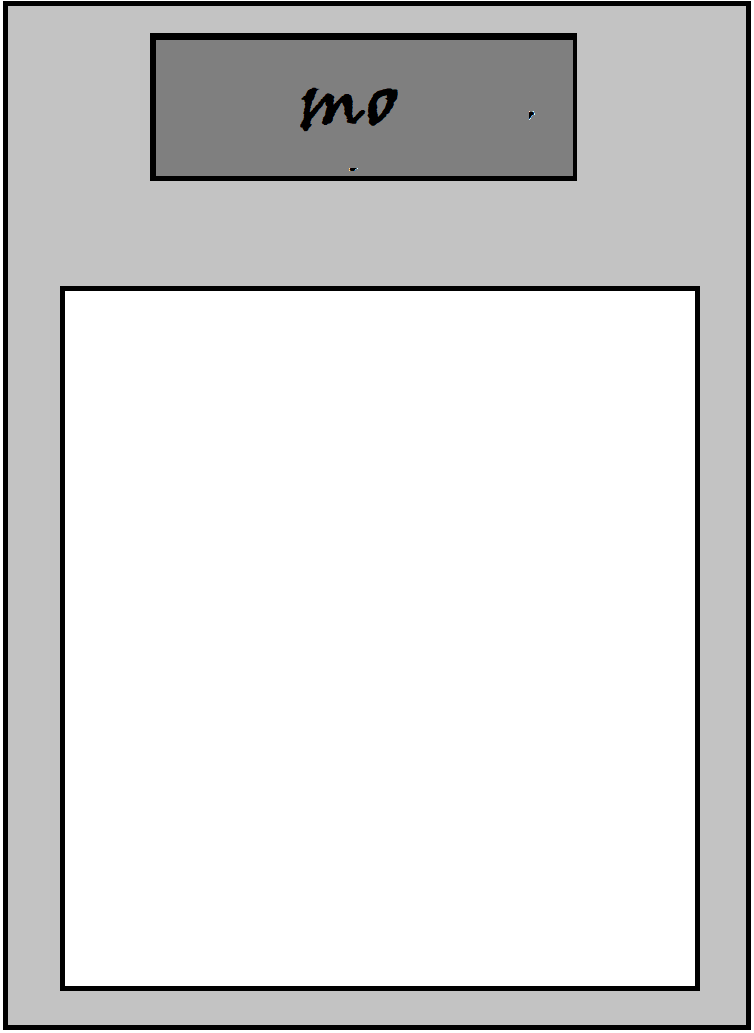
\includegraphics[width=\linewidth]{draw.png}
      \caption{Wizualizacja okna z trybem gry ,,DrawIt''}
    \end{subfigure}
    \begin{subfigure}[b]{0.35\linewidth}
      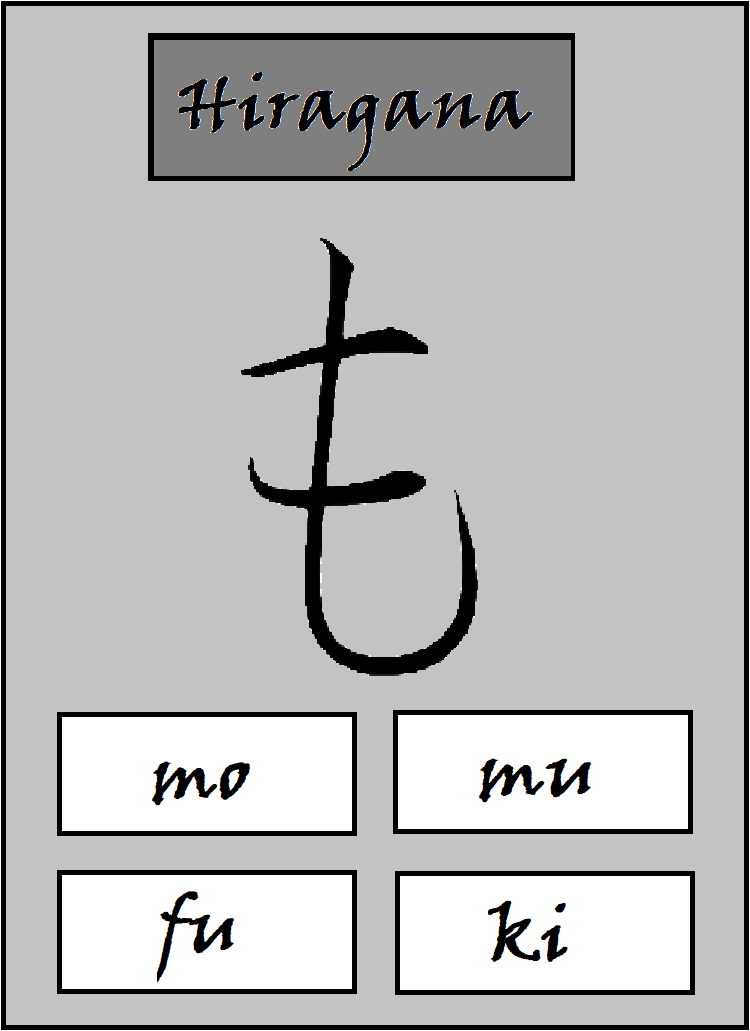
\includegraphics[width=\linewidth]{guess.png}
      \caption{Wizualizacja okna z trybem gry ,,GuessIt''}
    \end{subfigure}
    \label{fig:coffee}
  \end{figure}

  
  \subsection{Scena trybu,,GuessIt''}
  
  Scena reprezentująca drugi tryb gry (rysunek 2b). Składać się będzie z jednego imageview zawierającego obraz z danym znakiem, jednego textview z nazwą systemu znakowego oraz czterema przyciskami. Każdy z tych przycisków zawierać będzie 4 nazwy znaków z czego tylko jedna będzie prawidłowa. Wciśnięcie poprawnego przycisku będzie dodawało punkty do ogólnej sumy.
  
  \subsection{Scena podsumowania}
  Ta scena będzie wyświetlana po ukończeniu rozgrywki w obojętnie którym trybie (rysunek 3a). Zawierać będzie textview z podsumowaniem punktów oraz dodatkowo, jeżeli została wyświetlona po trybie ,,DrawIt'', będzie zawierała jeszcze elementy typu imageview przedstawiające narysowane przez użytkownika znaki.
  
  
  \begin{figure}[h!]
    \centering
    \begin{subfigure}[b]{0.35\linewidth}
      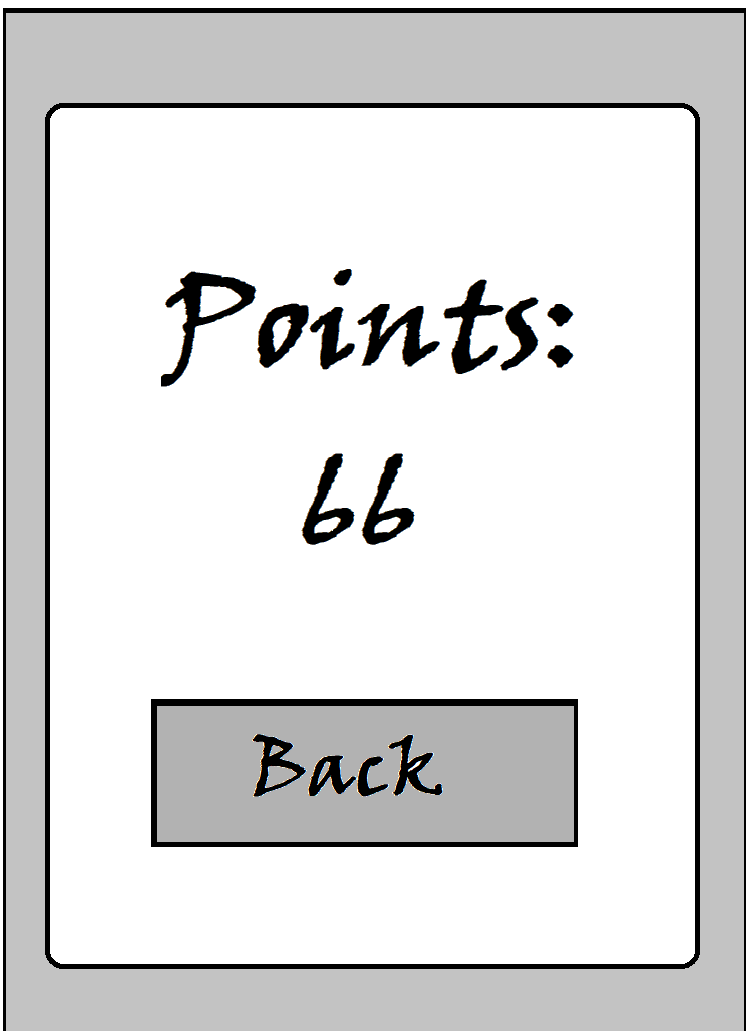
\includegraphics[width=\linewidth]{points.png}
      \caption{Wizualizacja okna z podsumowaniem.}
    \end{subfigure}
    \begin{subfigure}[b]{0.35\linewidth}
      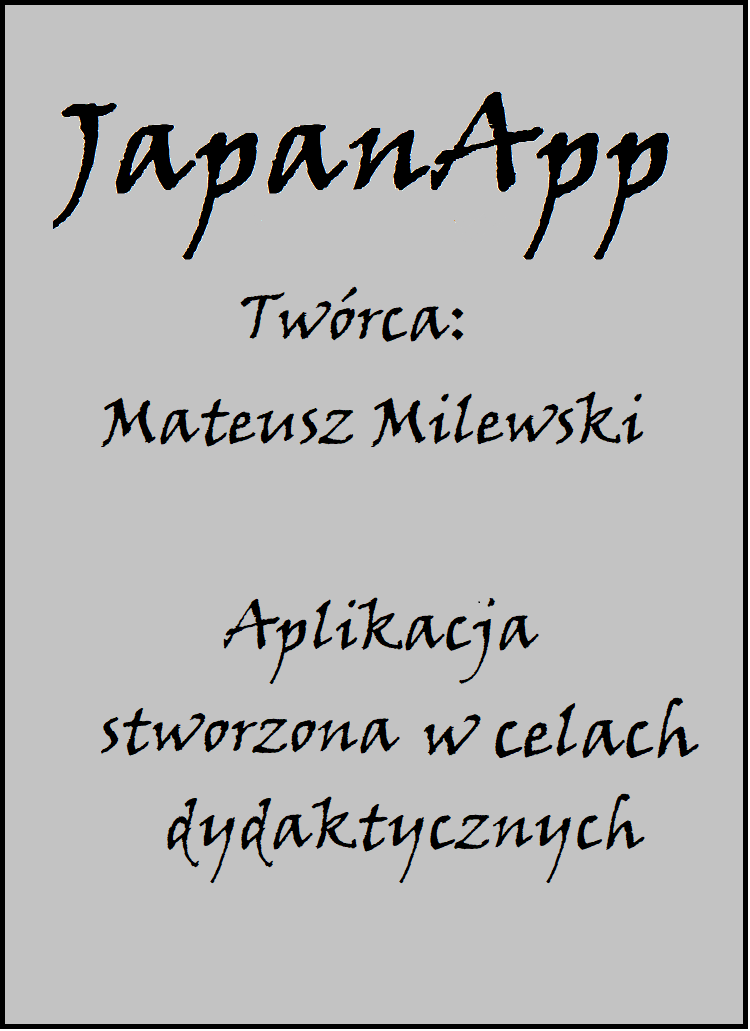
\includegraphics[width=\linewidth]{credits.png}
      \caption{Wizualizacja okna z informacjami od twórców.}
    \end{subfigure}
    \label{fig:coffee}
  \end{figure}
  
  \newpage
  \subsection{Scena z informacjami od twórców}
  Przeniesieni na nią zostaniemy po wciśnięciu przez użytkownika przycisku ,,credits'' w menu głównym (rysunek 3b). Scena ta składać się będzie z dwóch elementów typu textview, w których będą zawarte informacje od twórców (cel aplikacji, imię i nazwisko twórcy).
  
  \section{Opis klas}
  
  \subsection{Opis}
  Wszystkie klasy posiadają podobną strukturę. Atrybutami są odpowiednie przyciski i pola tekstowe, natomiast metody każda z nich przesłania takie same (onCreate(), onPause(), onStop(), onDestroy(), onResume(), onRestart(), onStart()). Przy wykorzystaniu tych metod aplikacja będzie kontrolować swoje działanie, jeżeli użytkownik zdecyduje się ją opuścić, zamknąć lub schować.
 
  \subsection{Diagram}
  Poniżej przedstawiony jest diagram, na którym zaprezentowane są klasy wraz z atrybutami i relacjami między nimi. Obiekty zwierające fragment ,,XML File'' w nazwie to pliki zawierające reprezentację graficzną odpowiednich scen.
  \begin{figure}
    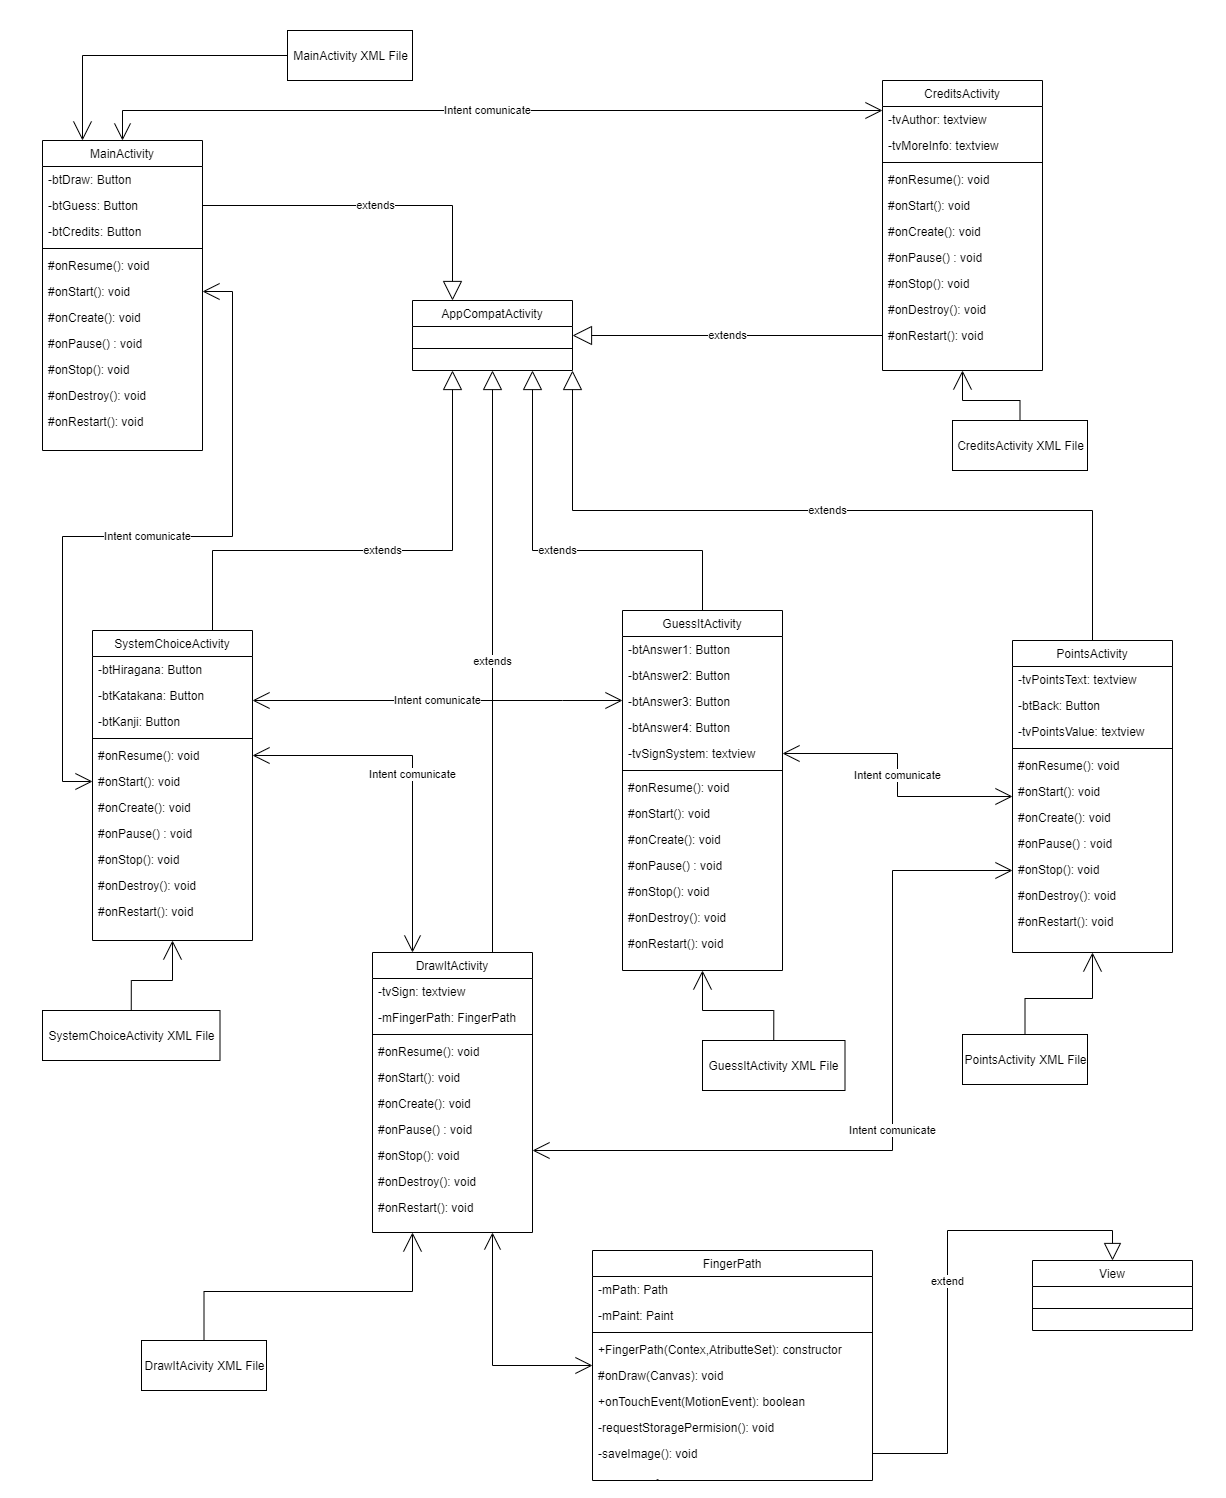
\includegraphics[width=\linewidth]{diagram}
    \caption{Diagram klas.}
    \label{fig:diagram}
  \end{figure}

  \newpage
  \subsubsection{MainActivity}
  Klasa reprezentująca scenę z menu głównym. Metoda onCreate() na starcie przypisywać będzie do każdego z przycisków ich onClickListenerów, odpowiadających za działanie przycisków. Dodatkowo dla przycisków ,,DrawIt'' oraz ,,GuessIt'', będzie ustawiała odpowiedni intent. Zawartość jego będzie przekazywana poprzez metodę intent.putExtra() do klasy z wyborem systemu znakowego. Pozostałe metody zostaną przesłonięte lub nie. Zależeć to będzie od zachowania aplikacji po pierwszych testach. Jeżeli aplikacja będzie posiadać problemy w sytuacji, kiedy użytkownik zostawi ją pracującą w tle i następnie do niej wrócił to przesłaniana będzie metoda onStop() w celu naprawienia błędu. Analogiczny schemat będzie dotyczył pozostałych metod w pozostałych klasach. 
  \subsubsection{SystemChoiceActivity}
  Klasa zarządzająca funkcjonalnością sceny z wyborem systemu znakowego. W Metodzie onCreate()  analogicznie jak poprzednio ustawiamy onClickListenerów, a następnie odbieramy informacje od poprzedniej klasy, przy pomocy metody intent.getExtra(). Na podstawie tych informacji zostanie otwarta scena z odpowiednią rozgrywką. 
  
  \subsubsection{DrawActivity}
  DrawActivity w raz z klasą FingerPath reprezentują scenę z rozgrywką w trybie ,,DrawIt''. W metodzie onCreate() na starcie wylosowane zostanie 20 nazw znaków z odpowiedniego systemu znakowego. Następnie przypisywana będzie jedna z tych nazw do textview oraz dodawany będzie obiekt klasy FingerPath reprezentujący pole do rysowania palcem po ekranie. Po zatwierdzeniu rysunku schemat ten będzie powtarzany dla nowego znaku.
  
  \subsubsection{FingerPath}
  Jest to klasa rozszerzająca podstawową klasę View, w celu stworzenia fragmentu okna na którym użytkownik może rysować po ekranie. W konstruktorze tej klasy będą ustawiane podstawowe wartości pędzla jak kolor, szerokość, style itp. Metoda onDraw() będzie odpowiadała za rysowanie już po wyznaczonej ścieżce przy pomocy biblioteki Canvas. Ścieżka palca będzie na bieżąco modyfikowana w metodzie onTouchEvent(). Podczas zamykania tego okna będą uruchamiane dwie metody requestStoragePermission(), w celu zdobycia dostępu do pamięci oraz metoda saveImage(), zapisująca rysunek w pliku png.
  
  \subsubsection{GuessActivity}
  Jest to druga z klas reprezentujących rozgrywkę tym razem w trybie ,,GuessIt''. Podobnie jak poprzednio na starcie w metodzie onCreate() losowane są 4 pary (nazwa znaku i rysunek znaku). Następnie z tych czterech par losujemy jedną jako tą prawdziwą i jej rysunek dodajemy do imageview. W zależności od udzielonej odpowiedzi dodawane lub odejmowane są punkty. Ten schemat z losowaniem i przypisywaniem powtarzany jest 20 razy.
  
  \newpage
  \subsubsection{PointsActivity}
  Klasa z podsumowaniem wyników z rozgrywki. Metoda onCreate() pobiera za pomocą intent.getExtra() sumę zdobytych punktów z rozgrywki i dodaje ją do textview. W przypadku trybu ,,DrawIt'' dodatkowo pobierane są wcześniej narysowane znaki i również wyświtlane w oknie podsumowania. 
  
  \subsubsection{CreditsActiity}
  Ostatnia z klas zawiera już same informacje od twórców. W metodzie onCreate() zostanie ustawiony tylko tekst jaki mają wyświetlać poszczególne textview. 
  
  \section{Testowanie}
  \subsection{Konwencja nazewnictwa}
  Mając na celu posiadanie czytelnej informacji à propos tego co dane metody będą testować, zostanie przyjęta pewna konwencja.
  \newline
  \newline
  \textbf{[Test][nazwa sprawdzanej metody][jaki powinien być jej efekt]}
  \newline
  \newline
  np. test dla metody ,,generateRandomAnswer'' generującej 3 losowe błędne odpowiedzi do trybu ,,guessIt'', będzie miał nazwę ,,testGenerateRandomAnswerCheckIncorrectnesOfAnswers''.
  \subsection{Rodzaje testów}
  Poprawność działania aplikacji będzie testowana na kilku poziomach:
  \begin{enumerate}
    \item Testowanie przy pomocy testów jednostkowych do kluczowych metod za pomocą biblioteki JUnit.
    \item Testowanie wydajności działania aplikacji poprzez przeprowadzanie rozgrywek na różnych telefonach i w różnych trybach nauki.
  \end{enumerate}
  
  \end{document}
  